\section{VHF/UHF展開アンテナ(仁尾・坂本)}

\subsection{概要}
下図に示すVHF/UHFの展開アンテナを新規で開発した.JAXA文書「CSA-112040A 小型衛星非金属ロックワイヤに関する安全チェックリスト」に準拠する設計とした.
\begin{figure}[H] 
	\centering
	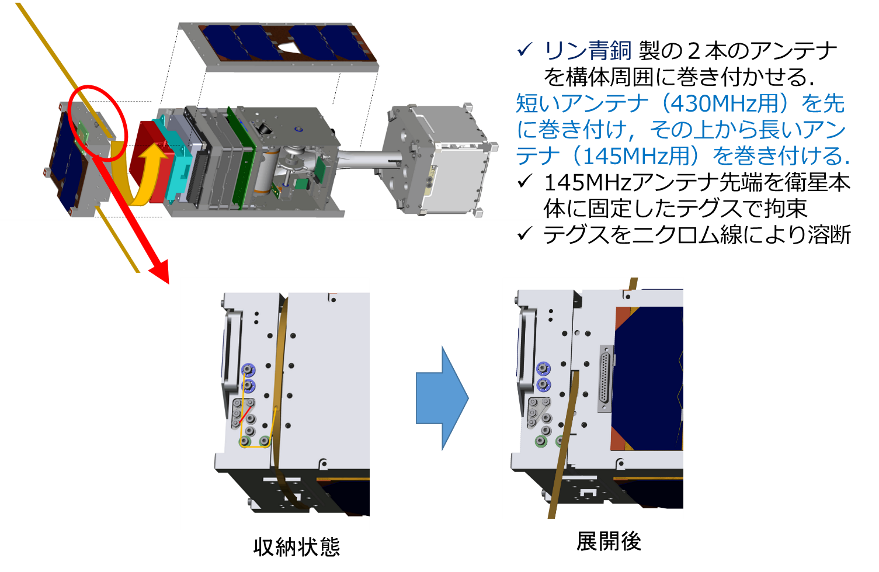
\includegraphics[scale=1]{03/fig/3-8-1.png}
	\caption{VHF/UHF展開アンテナの概要}
	\label{fig3-8-1}
\end{figure}
\begin{figure}[H]
		\centering
		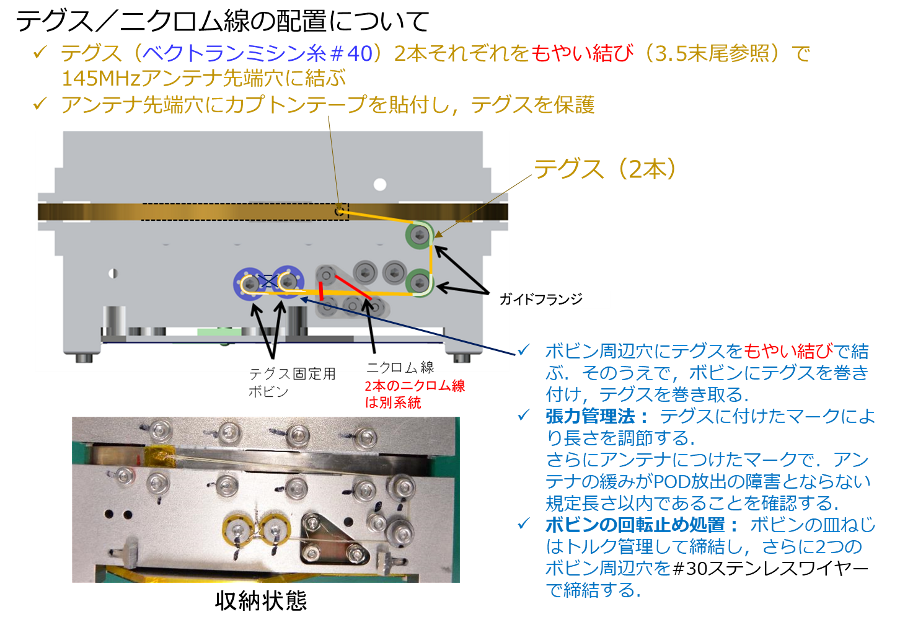
\includegraphics[scale=1]{03/fig/3-8-2.png}
	\caption{VHF/UHF展開アンテナのテグスとニクロム線配置}
	\label{fig3-8-2}
\end{figure}
\begin{figure}[H]
		\centering
		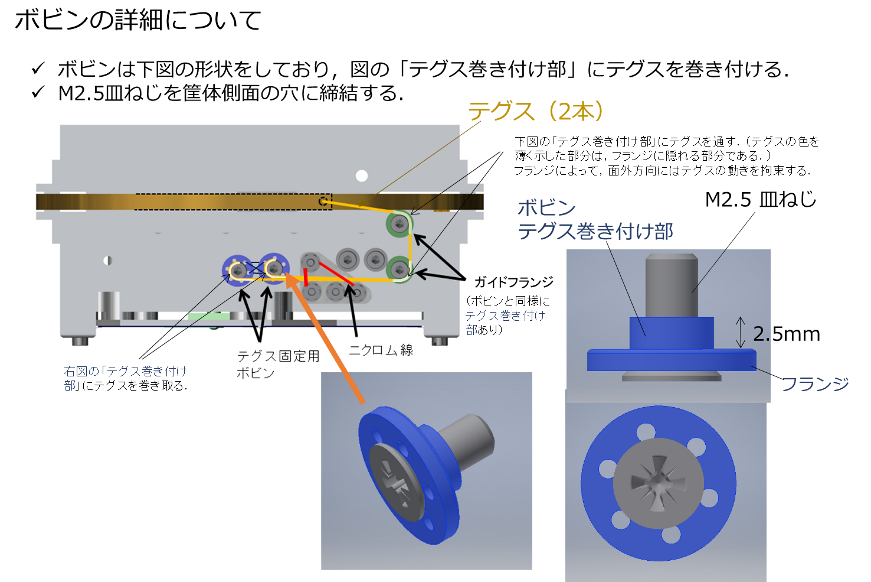
\includegraphics[scale=1]{03/fig/3-8-3.png}
	\caption{VHF/UHF展開アンテナのテグス用ボビン}
	\label{fig3-8-3}
\end{figure}
\begin{figure}[H]
		\centering
		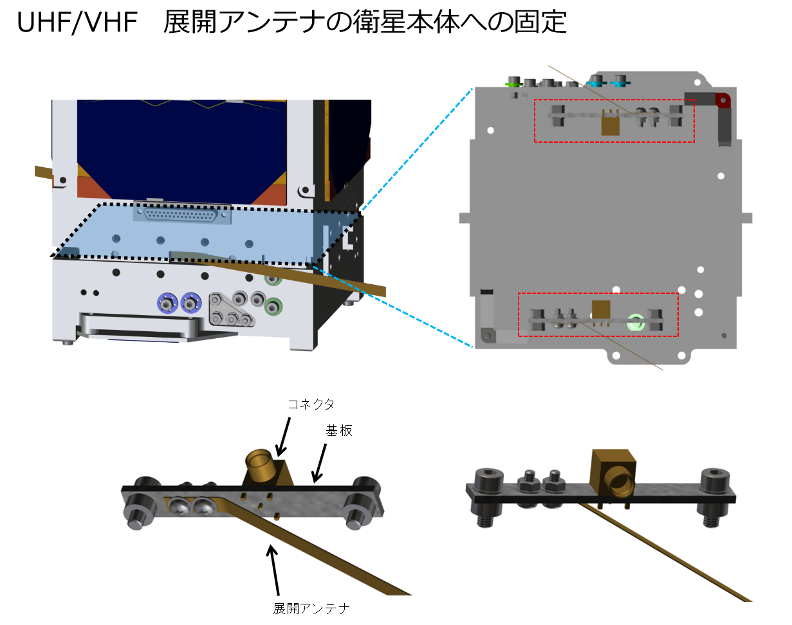
\includegraphics[scale=1]{03/fig/3-8-4.png}
	\caption{VHF/UHF展開アンテナの本体への固定}
	\label{fig3-8-4}
\end{figure}

\subsection{アンテナ材料の選定と製造}CSA-112040A 
2015年9月から開発を開始した.展開機構・回路は,日本大学SEEDSとSPROUTの経験を基盤とし,材料としてリン青銅を選択した.
しかし,収納試験を行ったところ,曲げ癖により展開後の真直度が低かった.そこで大阪府立大学OPUSATの経験を聞いたところ,バネ性リン青銅をコンベックス(巻き尺)形状に加工する特注品を作っていたということだった.
府立大衛星チームからの紹介で阿尾システムエナジー研究所(担当:阿尾様)に試作を依頼したところ,真直度の向上が見られたため,この特注アンテナを採用した.寸法などの詳細は以下である.インピーダンスマッチングを行って長さを調整するためにアンテナは長めに製作した.
価格は2本+2本で約11万円であった.
\begin{itemize}
	\item 加工依頼内容: コンベックスR形状の加工
	\item 材料: バネ性リン青銅(C5210P-H)
	\item 寸法と個数:(長さx幅x厚さ)= 300x5x0.1mm および 700x5x0.1m  
\end{itemize}
コンベックスR加工したものは高価であったため,コンベックス加工していない同材料のアンテナ(数千円)を試験用に購入し,限定的な数のみコンベックスR加工品を購入した.
 
\subsection{テグス,ニクロム線,ボビン}
テグスおよびボビンは,サカセ・アドテック社が開発した「膜展開部」の溶断機構と同一のものを用いることとした.ニクロム線は日本大などの設計を基に自作した.

\subsection{金メッキ}
バネ性リン青銅の錆を防止するため,FMについてはアンテナ全体に金メッキを施した.以下に手順を示す.

試験道具は以下である.
\begin{itemize}
	\item メッキ工房金メッキセット(https://www.higasi-osaka.com/mekki-koubou-senyou.htm)
	\item 金属磨き用ウエス
	\item 手袋
	\item メッキ用シート
	\item UHF/VHF展開アンテナ
\end{itemize}
試験手順は以下である.
\begin{enumerate}
	\item 購入後初の試験であったら,メッキ液の入った容器に穴をあけ,使える状態にする.
	\item メッキ用シートを敷く.
	\item 金属磨き:	金属磨き液をウエスに染み込ませ,十分光沢が出るまでメッキを行う金属を磨く.以降の作業は手袋を着用すること.
	\item 脱脂:	白色フェルトに脱脂液をしみこませ,メッキを行う金属の油分を十分取り除く.
	\item ニッケルメッキ:	緑色フェルトにニッケルメッキ液を染み込ませ,メッキを行う金属に十分に染み込ませる.十分に染み込ませたら,ニッケルメッキ液が乾くまでしばらく待つ.
	\item 金メッキ:	黄色フェルトに金メッキ液を染み込ませ,メッキを行う金属に十分に染み込ませる.
\end{enumerate}

ただし,少々の錆では通信機能に影響はない可能性もあり,この金メッキについては省くことができたかもしれない.

\subsection{開発と試験}

2015年9月から開発着手したものの,実質的なプロトタイプ製作は2017年1月ごろから開始された.

\noindent 2017/01/21:3Dプリンタ筐体を用いた収納・展開試験
\begin{figure}[H]
	\centering
	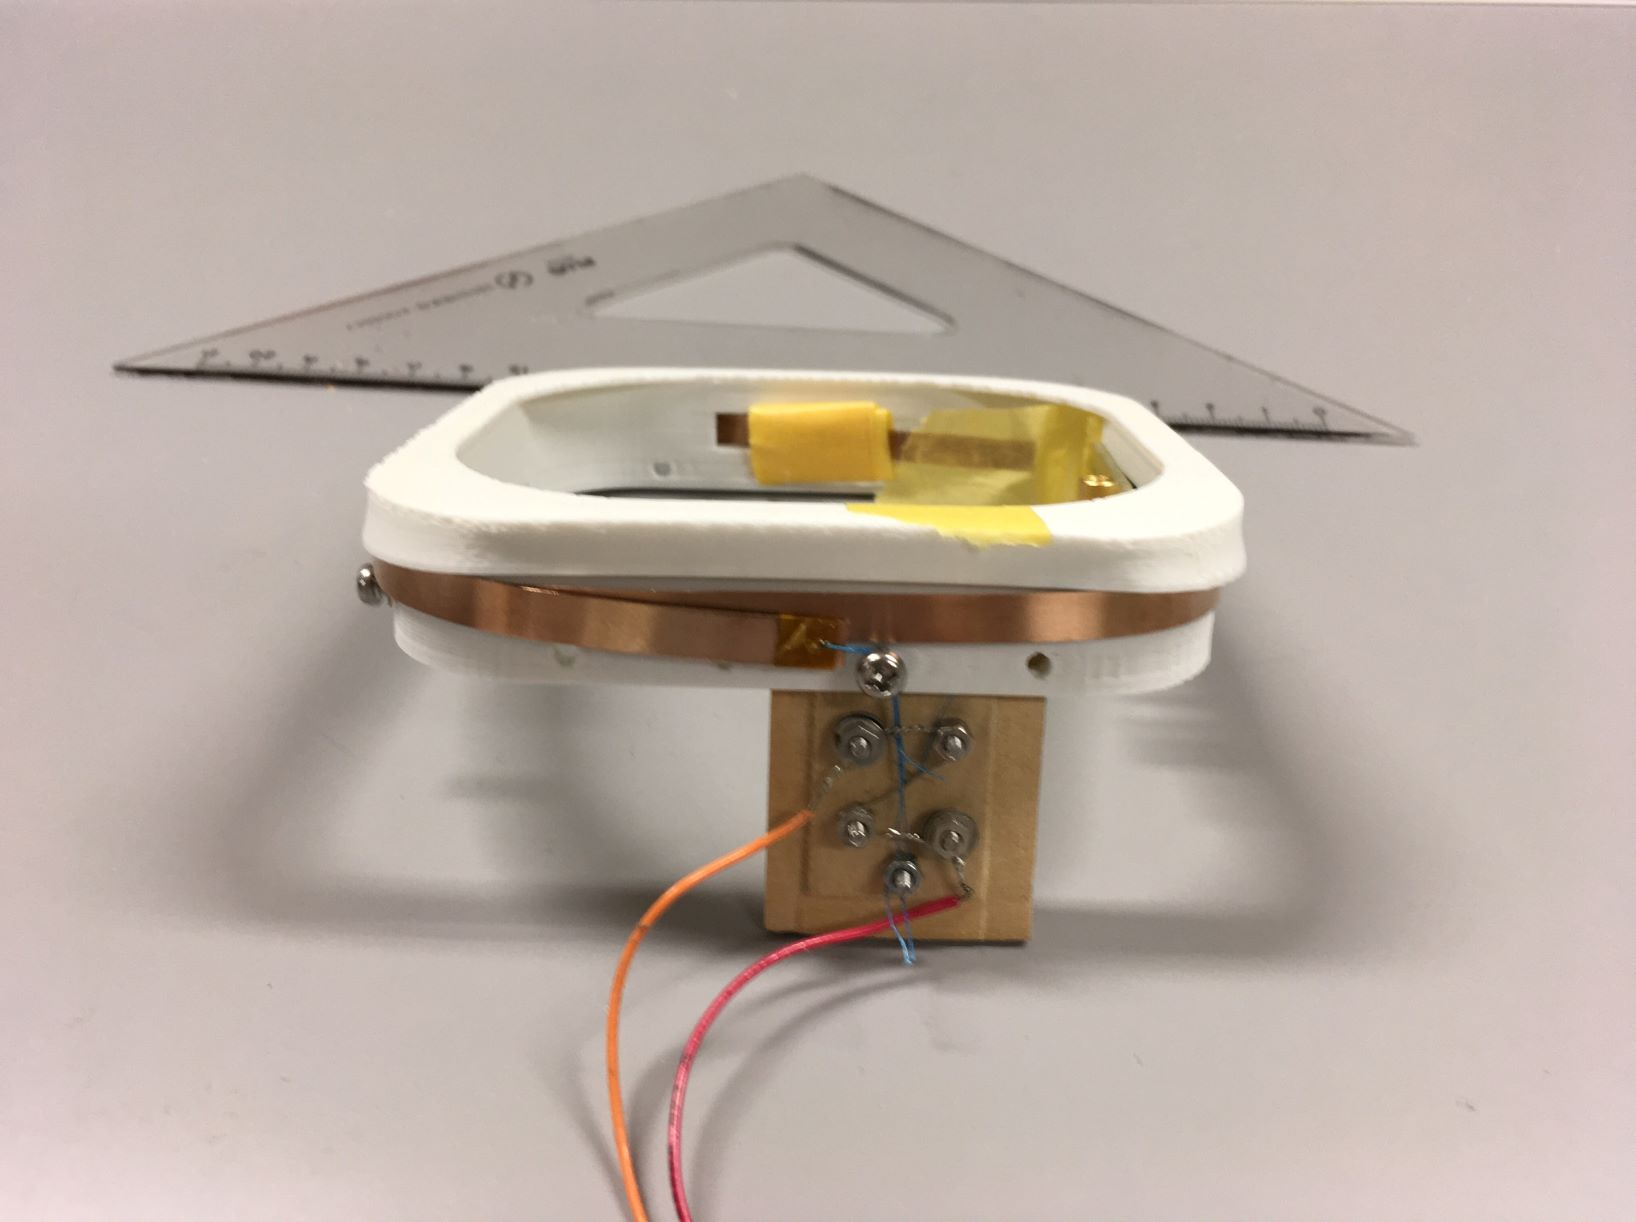
\includegraphics[width=0.5\textwidth]{03/fig/3-8-5.jpg}
	\caption{VHF/UHF展開アンテナ初期プロトタイプ収納・展開}
	\label{fig3-8-5}
\end{figure}

\noindent 2017/1/31:BBM溶断試験

電流値を変化させて溶断できる最小の電流値を探索した.BBM溶断回路(0.96Ω)に,
1.5Aだと溶断できず,1.8Aにて溶断成功した.1.8A流す設計として,抵抗値を調整した.
\begin{figure}[H]
	\centering
	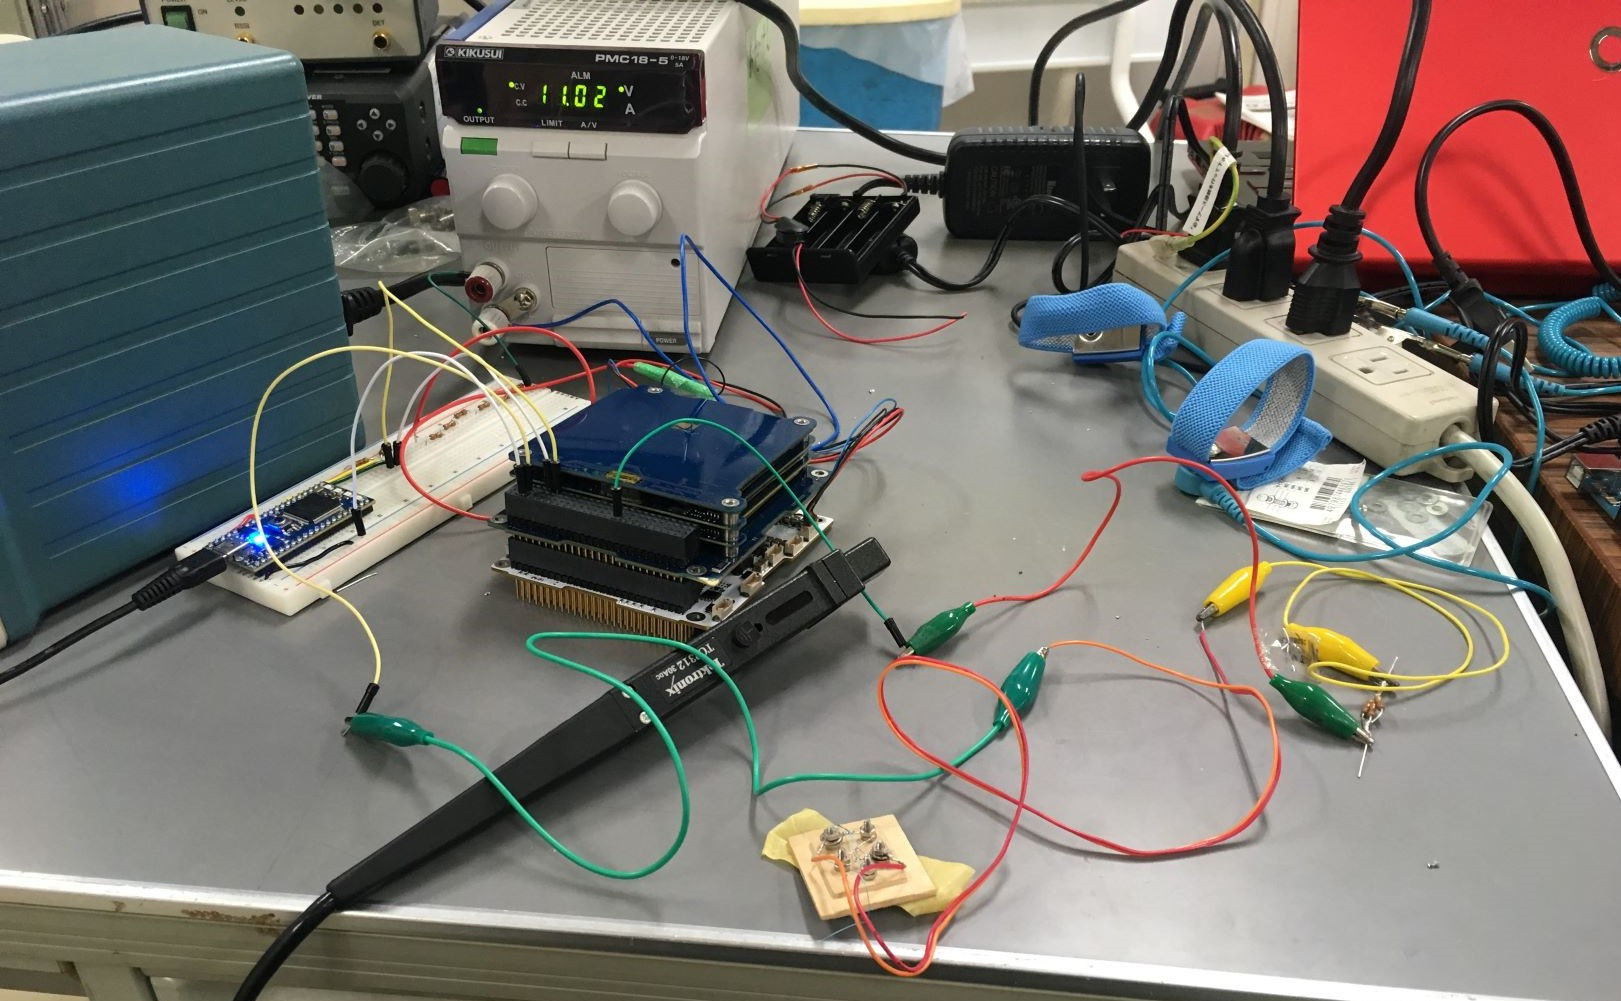
\includegraphics[width=0.5\textwidth]{03/fig/3-8-6.jpg}
	\caption{VHF/UHF展開アンテナ溶断回路BBM試験}
	\label{fig3-8-6}
\end{figure}

\noindent 2017/3/3:ボビンを模擬した溶断回路BBM2による溶断試験

電流値が2.0Aを下回り衛星EPS電源で溶断できることが確認できた.
今後溶断回路のバージョンアップによって抵抗値は変化する.その際は全体の抵抗値を3.3V/1.8A=1.83Ωにする方針を確認.
テグスがボビンに絡まる不具合があった.テグスの端部の取り扱いに注意.JAXAの衛星要求外形寸法(113mm*113mm)からはみ出しているため改善の必要あり(後日4/8のコンベックス加工をしたアンテナの収納試験で解消).

\begin{figure}[H]
	\centering
	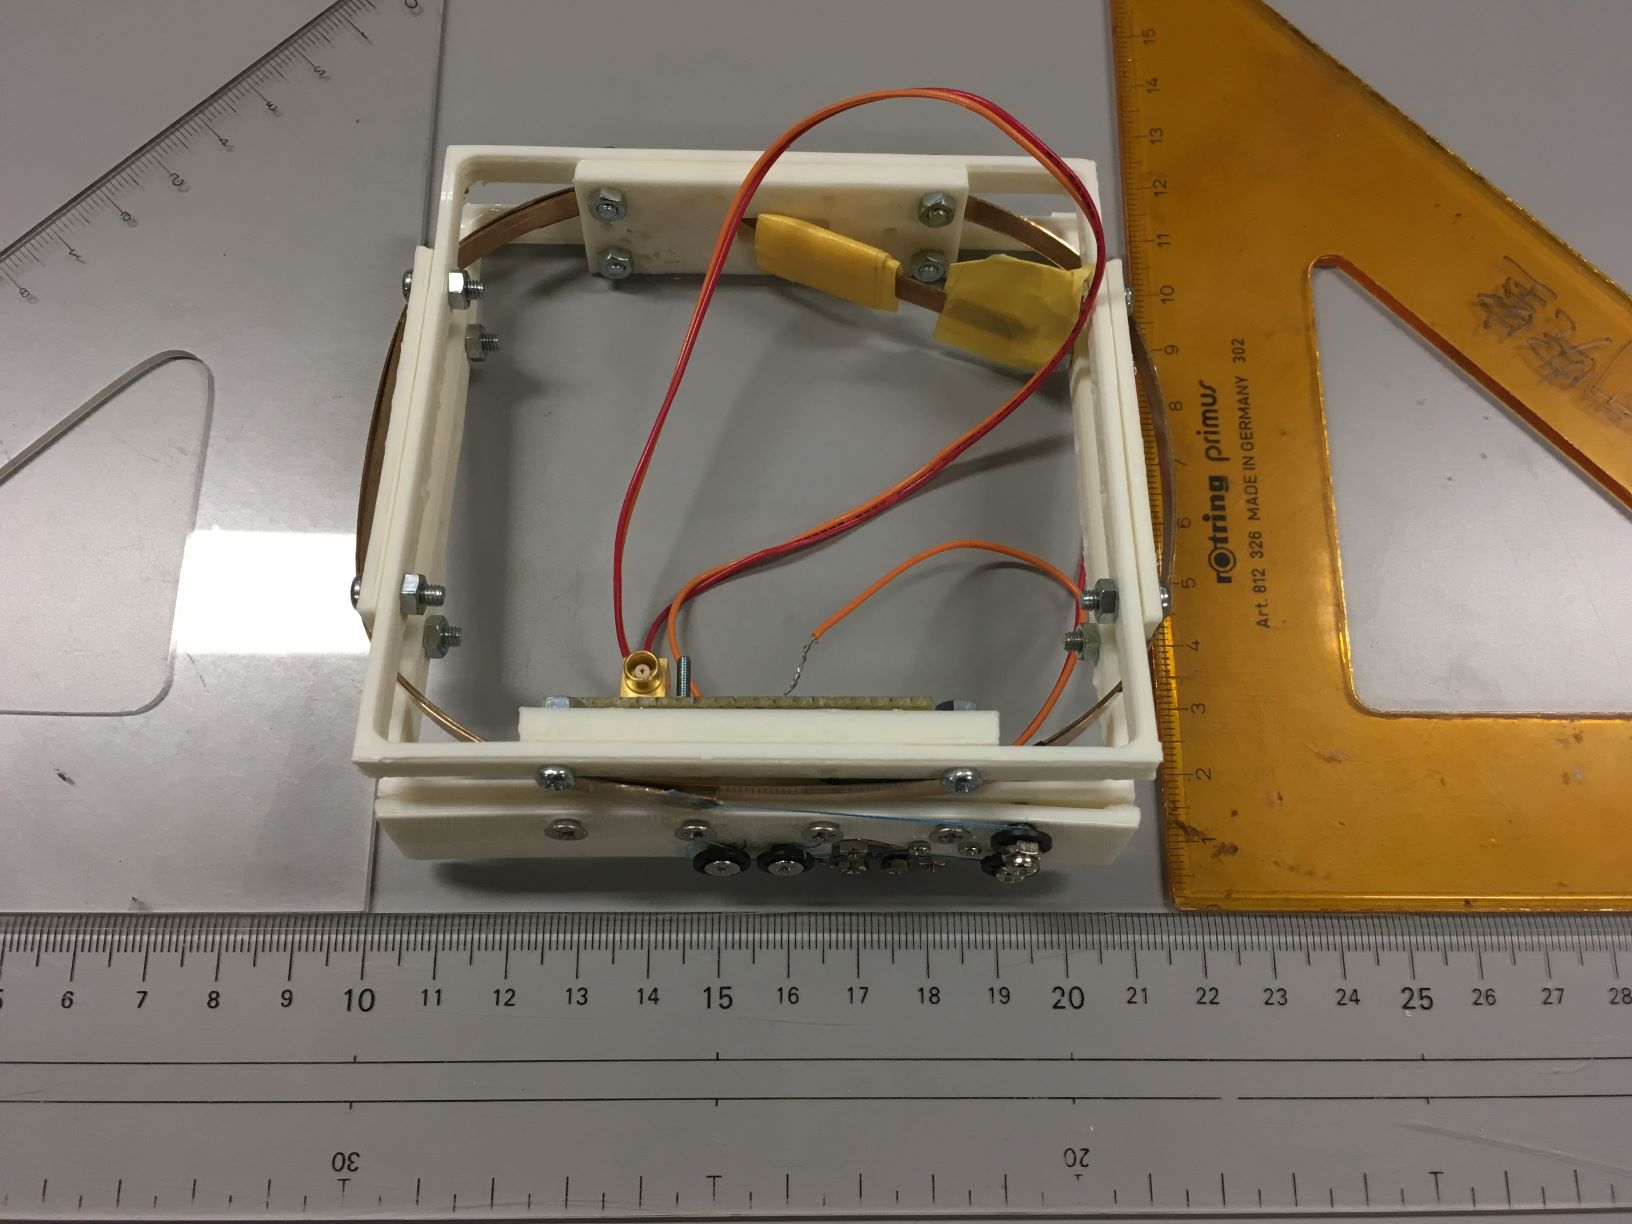
\includegraphics[width=0.5\textwidth]{03/fig/3-8-7.jpg}
	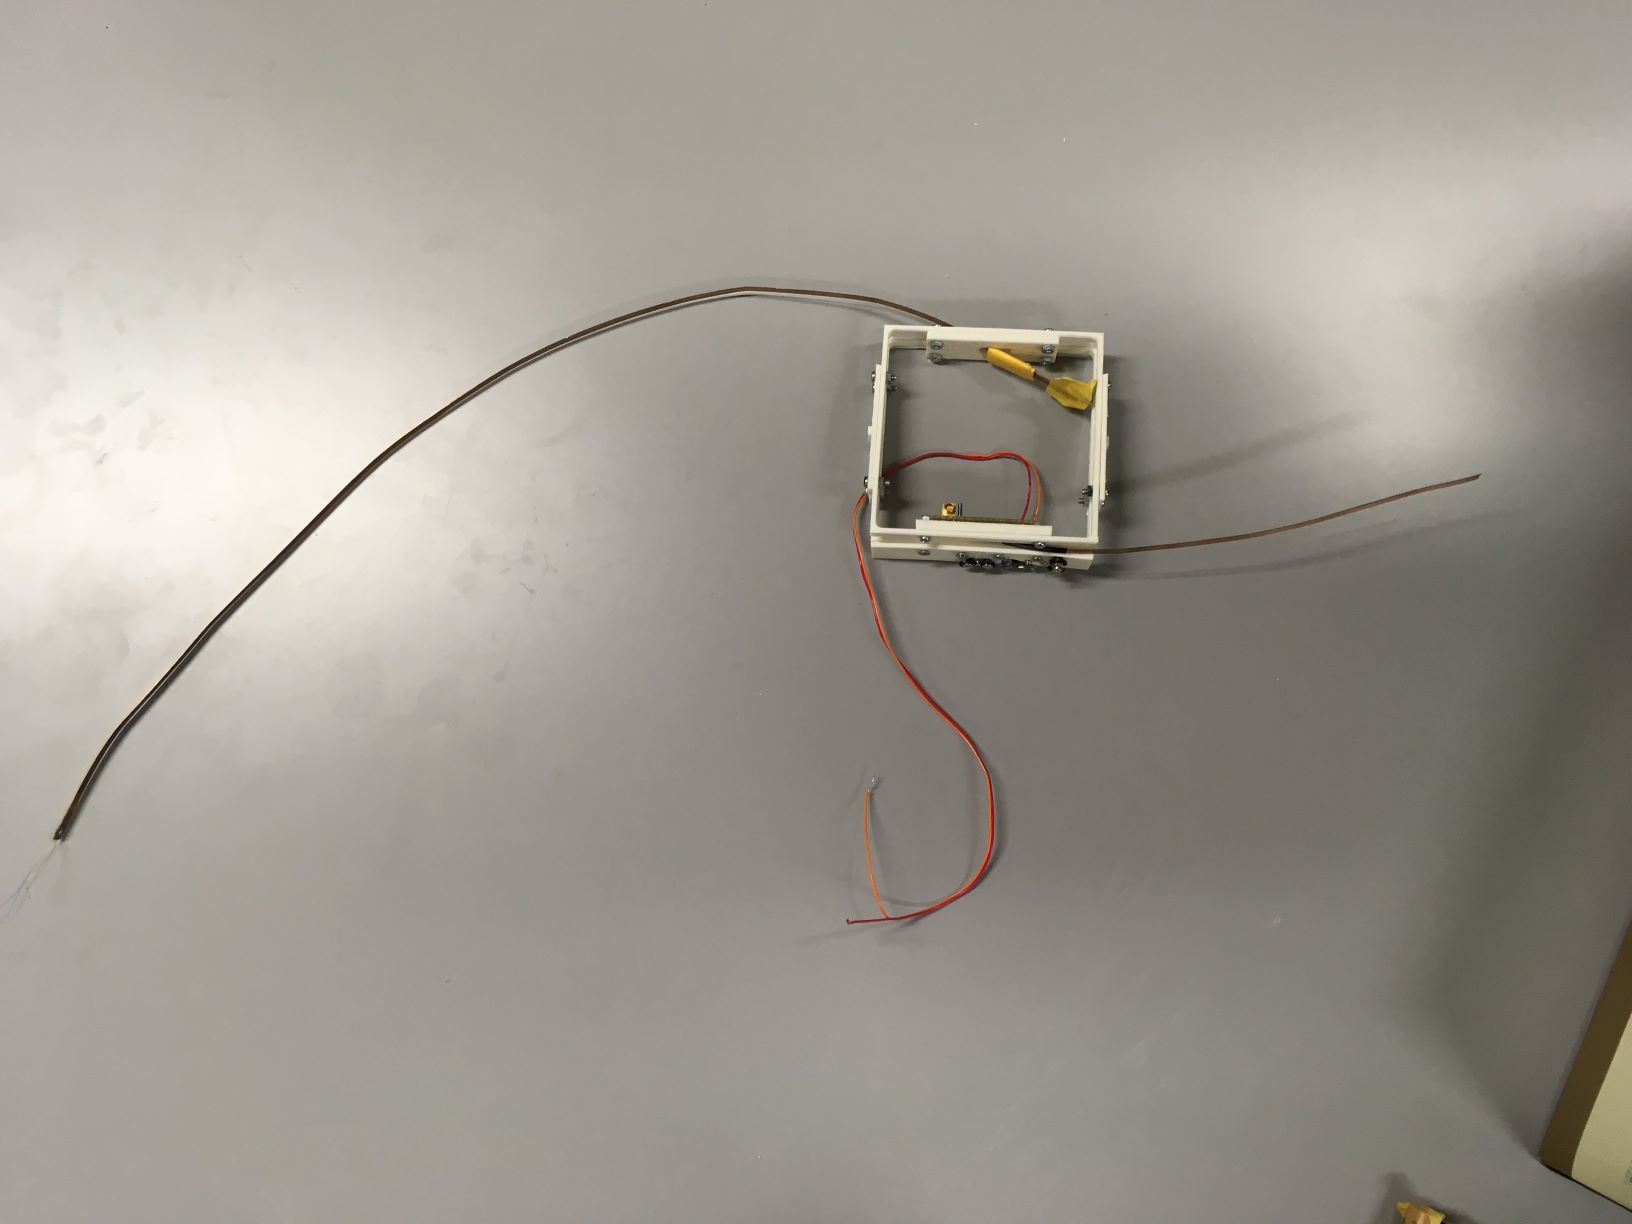
\includegraphics[width=0.5\textwidth]{03/fig/3-8-8.jpg}
	\caption{VHF/UHF展開アンテナ溶断回路BBM2試験}
	\label{fig3-8-8}
\end{figure}

\noindent 2017/7/1:恒温槽内での溶断試験
-65degに設定した恒温槽の内部でニクロム線0.1mm,0.2mm,0.4mmの三種類,テグスとしてダイニーマ0.8号,ベクトラン40号の二種類,それぞれ6種類の組み合わせにおいて溶断可能な電流値を測定した.テグスへの張力はM5ナットの重力によって与えた.恒温槽内の温度は-61.3degだった.
\begin{figure}[H]
	\centering
	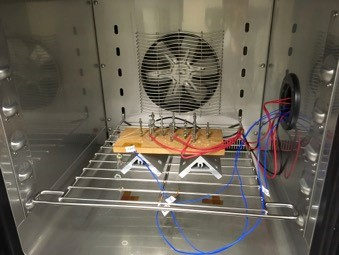
\includegraphics[scale=1]{03/fig/3-8-11.jpg}
	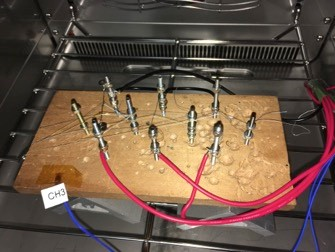
\includegraphics[scale=1]{03/fig/3-8-12.jpg}
		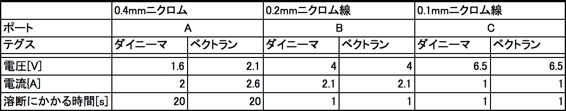
\includegraphics[scale=1]{03/fig/3-8-13.jpg}
	\caption{VHF/UHF展開アンテナ溶断回路の低温溶断試験}
	\label{fig3-8-13}
\end{figure}

\noindent 2018/1/5:長期収納試験

衛星構体形状と同一のモックアップに巻き付け収納時間の影響を計測した.
\begin{figure}[H]
	\centering
	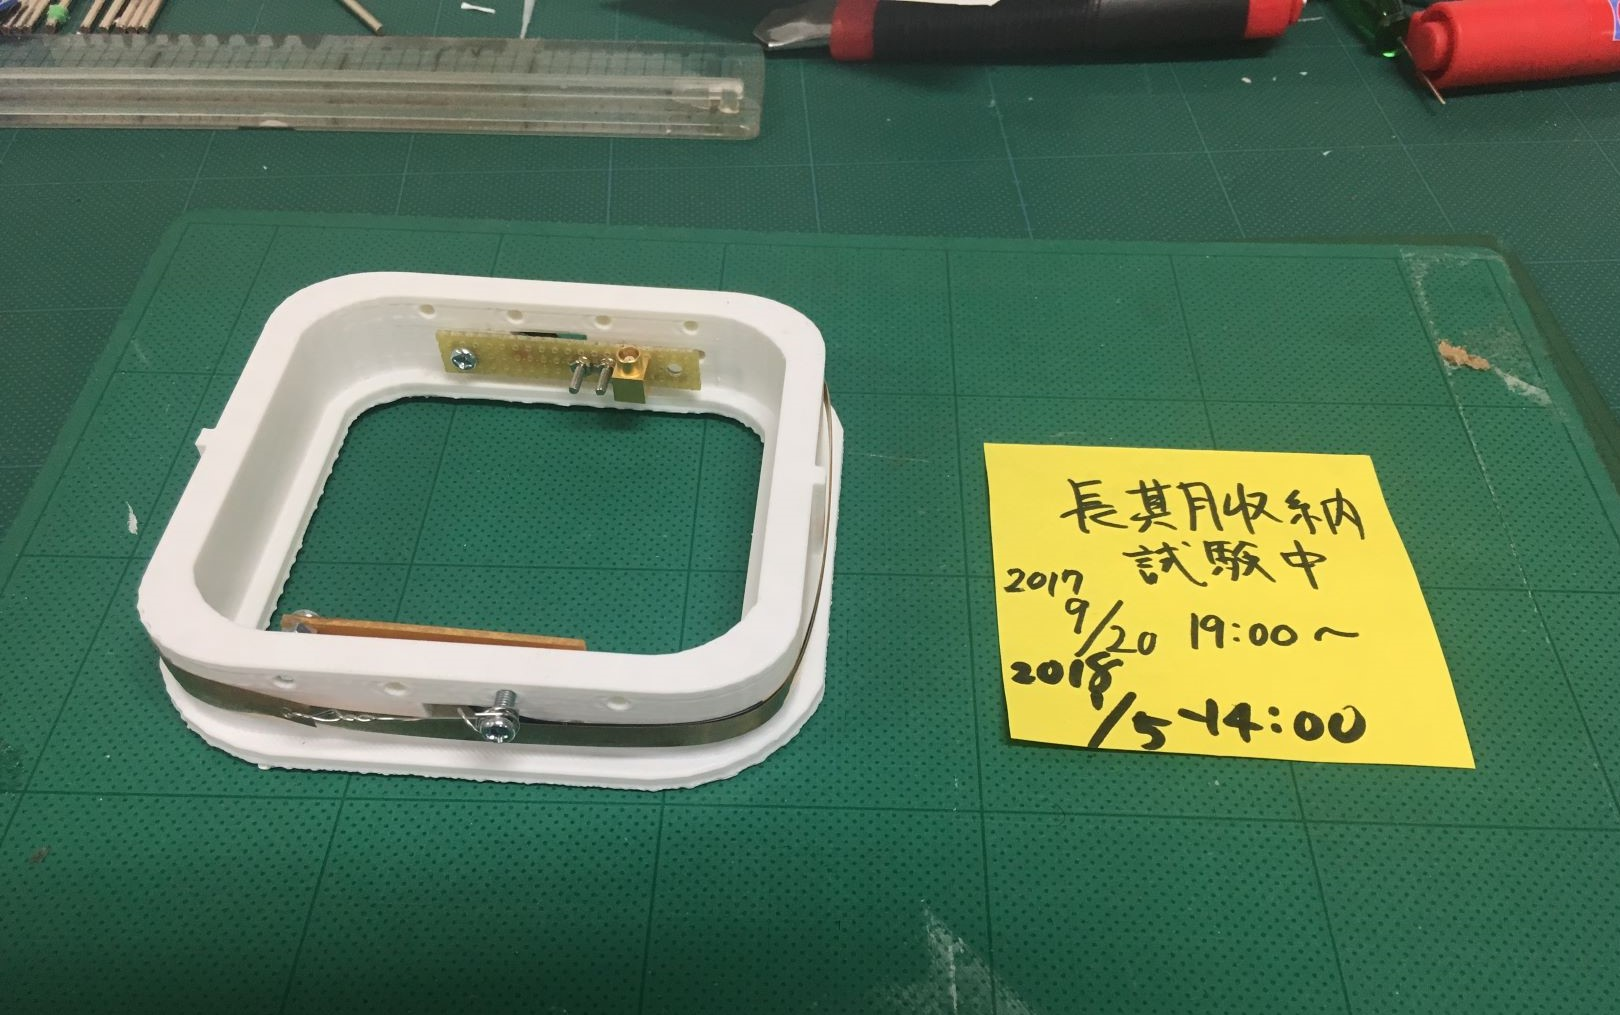
\includegraphics[width=0.5\textwidth]{03/fig/3-8-9b.jpg}
	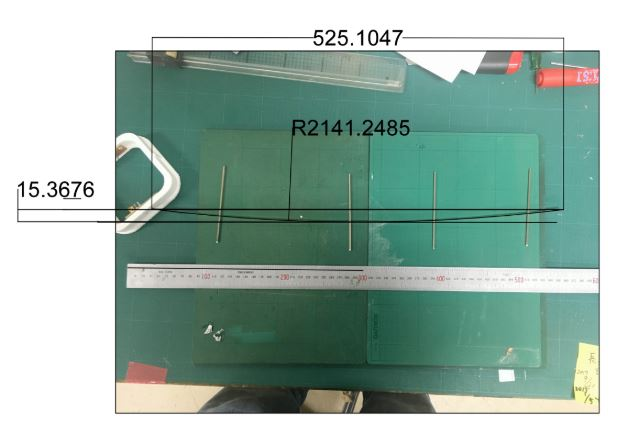
\includegraphics[width=0.5\textwidth]{03/fig/3-8-10.jpg}
	\caption{VHF/UHF展開アンテナ長期収納試験}
	\label{fig3-8-10}
\end{figure}

\subsection{収納手順}

組立て手順書を参照.FMの組み立てでは,展開アンテナの収納は最後の作業であり,作業者(仁尾)の待ち時間が非常に長かった.神経を使う作業であるのに呼ばれるタイミングが読めないでいた.

なお,フライト結果から,VHF/UHFアンテナは宇宙で正常に展開したことがわかっている.



